%&latex
%
\providecommand{\main}{../..}
\documentclass[../../main.tex]{subfiles}

\begin{document}

\subsection{Correlation function in the Mean Field}
\lesson{27}{11/05/20}
We want to verify (\ref{eqn:correlation-ansatz-full}) in the case of the mean field approximation. 

\medskip

So, we start with a \textit{separable} variational ansatz (\ref{eqn:mfi}, pag. \pageref{eqn:mfi}):
\begin{align} 
    \rho_0(\bm{\sigma}) = \prod_x \rho_x(\sigma_x) \qquad \rho_x(\sigma_x) = \frac{1+\textcolor{Blue}{m_x} \sigma_x}{2} \quad m_x \in [-1,1]
\end{align}
In this case, spins are independent, and so:
\begin{align*}
    \langle \sigma_x \sigma_y \rangle_0 = \sum_{\bm{\{\bm{\sigma}\}}} \rho_0(\bm{\sigma}) \sigma_x \sigma_y = \langle \sigma_x \rangle_0 \langle \sigma_y \rangle_0 \underset{(\ref{eqn:local-average})}{=} m_x m_y
\end{align*}
More in general, the $n$-point correlator between $m$ \textbf{distinct} $x_1, \dots, x_m$ spins is the product of the \textit{local magnetizations} $m_{x_i}$:
\begin{align*}
    \langle \sigma_{x_1} \cdots \sigma_{x_n} \rangle_0 = \prod_{i=1}^n m_{x_i}
\end{align*} 
This means that the correlation function $G_{xy}$ is trivial:
\begin{align*}
    G_{xy} \equiv \langle \sigma_x \sigma_y \rangle - \langle \sigma_x  \rangle \langle \sigma_y \rangle = m_x m_y - m_x m_y = 0
\end{align*}

A more interesting (and accurate) result can be obtained if we start from the \textbf{exact} partition function:
\begin{align*}
    Z(\bm{h}) = \sum_{\{\bm{\sigma}\}} \exp\left({-\beta H(\bm{\sigma}) + \sum_x h_x \sigma_x }\right)
\end{align*}
The magnetization $m_{x_i}$ at position $x_1$ can be obtained by deriving $\ln Z(\bm{h})$ with respect to the local field $h_{x_1}$ at that position (\ref{eqn:mag2}):
\begin{align*}
    \pdv{h_{x_1}} \ln Z(\bm{h}) = \frac{\displaystyle \sum_{\{\bm{\sigma}\}} \exp\left(-\beta H(\bm{\sigma}) + \sum_x h_x \sigma_x\right) \sigma_{x_1}}{Z(\bm{h})} = \langle \sigma_{x_1} \rangle = m_{x_1}
\end{align*}
And if we differentiate once more, with respect to $h_{x_2}$ with $x_2 \neq x_1$ (see the steps preceding (\ref{eqn:fluctuation_dissipation}) at pag. \pageref{eqn:fluctuation_dissipation}):
\begin{align*}
    \pdv[2]{}{h_{x_1}}{h_{x_2}} \ln Z(\bm{h}) &= \pdv{h_{x_1}} \langle \sigma_{x_1} \rangle = \frac{\displaystyle \sum_{\{\bm{\sigma}\}} \exp\left(-\beta H(\bm{\sigma}) + \sum_x h_x \sigma_x\right) \sigma_{x_1} \sigma_{x_2}}{Z} + \\
    &\quad \> -  \frac{\displaystyle \sum_{\{\bm{\sigma}\}} \exp\left(-\beta H(\bm{\sigma}) + \sum_x h_x \sigma_x\right) \sigma_{x_1}}{Z} \cdot \frac{\displaystyle \sum_{\{\bm{\sigma}\}} \exp\left(-\beta H(\bm{\sigma}) + \sum_x h_x \sigma_x\right) \sigma_{x_2}}{Z} =\\
    &= \langle \sigma_{x_1} \sigma_{x_2} \rangle - \langle \sigma_{x_1} \rangle \langle \sigma_{x_2} \rangle
\end{align*}
And so we get an exact result for the two-point correlation function:
\begin{align}\label{eqn:twop}
    G_{x_1 x_2} \equiv \pdv{m_{x_1}}{h_{x_2}} = \langle \sigma_{x_1}  \sigma_{x_2}\rangle - \langle \sigma_{x_1} \rangle \langle \sigma_{x_2} \rangle
\end{align}

In the mean field, local magnetizations obey equation (\ref{eqn:variational-sol}):
\begin{align}
    \label{eqn:var-sol2}
    m_x(\bm{h}, K) = \tanh \left[K \sum_{y \in \langle y, x\rangle} m_y + h_x\right]
\end{align}
where the sum is over all nodes $y$ that are neighbours of $x$. Solving for $h_x$ leads to:
\begin{align}\label{eqn:hx-step}
    h_x = \tanh^{-1} m_x - \sum_y K_{xy} m_y \qquad K_{xy} \underset{(a)}{\equiv}  K \delta_{|\bm{r}_x-\bm{r}_y|,a} = \begin{cases}
        K & |\bm{r}_x-\bm{r}_y|=a\\
        0 & \text{otherwise}
    \end{cases}
\end{align} 
Here we denote with $\bm{r}_x$ the position of node $x$ in the lattice, so that $|\bm{r}_x - \bm{r}_y|$ is the distance between spins $x$ and $y$. Neighbouring cells are separated only by the grid step $a$, and we use this fact to rewrite in (a) the sum over neighbours of $x$ as a sum over \textit{all nodes} by adding an appropriate Kronecker delta. 

\medskip

Differentiating both sides of (\ref{eqn:hx-step}) with respect to $h_z$ leads to:
\begin{align*}
\delta_{xz} &= \pdv{h_x}{h_z} = \frac{1}{1-m_x^2} \underbrace{\pdv{m_x}{h_z}}_{G_{xz} \> (\ref{eqn:twop})} - \sum_y K_{xy} \underbrace{\pdv{m_y}{h_z}}_{G_{yz}\>(\ref{eqn:twop})} =\\
&= \sum_y \underbrace{\left[\frac{\delta_{xy}}{1-m_x^2} - K_{xy} \right]}_{A_{xy}} G_{yz}
\end{align*}
This can be rewritten in matrix form as follows:
\begin{align}\label{eqn:AG-mtx}
    \mathbb{1} = \textbf{A} \textbf{G}
\end{align}
where the entries of $A$ are:
\begin{align*}
    \textbf{A}  = \resizebox{8cm}{!}{$\left(\begin{array}{cccc}
        \frac{1}{1-m_1^2}  - \cancel{K_{11}} & -K_{12} & -K_{13} & \cdots \\ 
        -K_{21} & \frac{1}{1-m_2^2}  - \cancel{K_{22}} & -K_{23} & \cdots \\ 
        -K_{31} & -K_{32} & \frac{1}{1-m_3^2}  - \cancel{K_{33}} & \cdots \\ 
        \vdots & \vdots & \vdots & \ddots
        \end{array}\right)$} \qquad A_{xy} = \frac{\delta_{xy}}{1-m_x^2} - K_{xy} 
\end{align*}
In the case of a \textbf{cubic lattice} with \textbf{periodic boundary conditions} the system is translationally invariant, and so it is reasonable to assume a \textbf{uniform magnetization}, i.e. $h_x \equiv h$ and $m_x \equiv m(h,T)$. This leads to:
\begin{align*}
    A_{xy} = \frac{\delta_{xy}}{1-m^2} - K_{xy} = \begin{cases}
        \frac{1}{1-m^2} & x=y\\
        -K & |\bm{r}_x-\bm{r}_y| = a 
    \end{cases} 
\end{align*}
And from (\ref{eqn:AG-mtx}) we obtain:
\begin{align}\label{eqn:G-mtx}
    \textbf{G}^{-1} = \textbf{A}  \Leftrightarrow (\textbf{G}^{-1})_{xy} = A_{xy} = \frac{\delta_{xy}}{1-m^2} - K_{xy} 
\end{align}
Note that the entries of $\textbf{G}^{-1}$ depend only on \textit{differences of positions} (in $K_{xy}$), meaning that $\textbf{G}^{-1}$ is translationally invariant. Explicitly, the (reciprocal of the) correlation between spins that are \textit{the same distance apart} is the same, and so:
\begin{align*}
    (\textbf{G}^{-1})_{xy} \equiv G^{-1}(\bm{r}_x, \bm{r}_y) = G^{-1}(\bm{r}_x + \bm{n}a, \bm{r}_y + \bm{n}a) \qquad \bm{n} \in \mathbb{Z}^d
\end{align*}  
Choosing $\bm{n}$ so that $\bm{r}_y = -\bm{n}a$ we get:
\begin{align}\label{eqn:corr_translational_invariance}
    G^{-1}(\bm{r}_x, \bm{r}_y) = G^{-1}(\bm{r}_x-\bm{r}_y,0) \equiv G^{-1}(\bm{r}_x - \bm{r}_y)
\end{align}
Translational invariance implies that $\textbf{G}^{-1}$ is diagonalized by the Fourier basis. 

\medskip

%See https://physics.stackexchange.com/questions/209191/translational-invariance-implying-diagonal-representation-in-momentum-space
This can be quickly\marginpar{Translational invariance and Fourier basis} shown in the \textit{continuum limit}, i.e. if we treat $\bm{r}_{x}$ and $\bm{r}_y$ as continuous variables. Then, ignoring the normalization constants: 
\begin{align} \label{eqn:fourier-basis1}
    \mathcal{F}[G^{-1}](\bm{p}, \bm{q}) 
    &\propto
    \int_{\mathbb{R}^d} \dd[d]{\bm{r}_x} e^{i \bm{p} \cdot \bm{r}_x} \int_{\mathbb{R}^d} e^{i \bm{q} \cdot \bm{r}_y}\hlc{Yellow}{G^{-1}(\bm{r}_x, \bm{r}_y)} = \\ \nonumber
    &\underset{(\ref{eqn:corr_translational_invariance})}{=}  \int_{\mathbb{R}^{2d}} \dd[d]{\bm{r}_x} \dd[d]{\bm{r}_y} e^{i \bm{p}\cdot \bm{r}_x} e^{i \bm{q}\cdot \bm{r}_y} \hlc{Yellow}{G^{-1}(\bm{r}_x - \bm{r}_y)} =\\ \nonumber
    &\underset{\mathclap{\bm{t} = \bm{r}_x - \bm{r}_y}}{=} \quad \int_{\mathbb{R}^{2d}} \dd[d]{\bm{t}} \dd[d]{\bm{r}_y} e^{i \bm{p} \cdot \bm{t}} e^{i \bm{r}_y \cdot (\bm{p} + \bm{q})} G^{-1}(\bm{t}) =\\ \nonumber
    &= \underbrace{\int_{\mathbb{R}^d} \dd[d]{\bm{t}} e^{i \bm{p} \cdot \bm{t}} G^{-1}(\bm{t})}_{\mathcal{F}[G^{-1}](\bm{p})} \underbrace{\int_{\mathbb{R}^d} \dd[d]{\bm{r}_y} e^{i \bm{r}_y \cdot (\bm{p} + \bm{q})}}_{\delta^d(\bm{p} + \bm{q})} = \tilde{G}^{-1}(\bm{p}) \delta^d(\bm{p} + \bm{q})
\end{align} 
And so $\mathcal{F}[G^{-1}](\bm{p}, \bm{q})$ can be nonzero only if $\bm{p} = -\bm{q}$, meaning that can be seen as a (infinite) diagonal matrix\footnote{A discrete matrix $\mathcal{M}_{N \times N}(\mathbb{R})$ is diagonal if it has entries $A_{xy} = A_{x} \delta_{xy}$. Here we have some sort of \q{continuous matrix} - which should really be intended as the matrix representation in the Fourier basis of a linear operator on $L^2(\mathbb{R}^d)$. So, in a sense, it is a $\infty \times \infty$ matrix \q{centred in $\bm{0}$}. In the $d=1$ case, it can be thought as of a \textit{plane}, with entries at every point $(p,q)$, and the diagonal being the second-fourth quadrant bisector $p=-q$.}. Then, the inverse of a diagonal matrix is obtained by replacing each element in the diagonal with its reciprocal:
\begin{align*}
    \mathcal{F}[G^{-1}](\bm{p}, \bm{q}) = \frac{1}{\mathcal{F}[G^{-1}](\bm{p})} \delta^{d}(\bm{p} + \bm{q}) 
\end{align*} 

However, $\bm{r}_x$ and $\bm{r}_y$ are constrained to \textbf{discrete} positions in the cubic lattice - in other words $G^{-1}(\bm{r}_x, \bm{r}_y)$ should really be a function $\mathbb{Z}^{d}\times \mathbb{Z}^d \to \mathbb{R}$. By adding some Dirac deltas, we can extend the domain to $\mathbb{R}^d \times \mathbb{R}^d$, essentially making the function vanish for all non-integers arguments:
\begin{align*}
    G^{-1}(\bm{r}_x, \bm{r}_y) = \sum_{\bm{n,m} \in \mathbb{Z}^d} G^{-1}(\bm{r}_x, \bm{r}_y) \delta^d(\bm{r}_x-\bm{n}a) \delta^d(\bm{r}_y - \bm{m} a) \qquad \bm{r}_x, \bm{r}_y \in \mathbb{R}^d
\end{align*}
$G^{-1}$ has a period of $a$ for all its arguments, and so its Fourier transform will have\footnote{See \url{https://www.gnu.org/software/gnuastro/manual/html_node/Dirac-delta-and-comb.html} for the proof.} a period of $2\pi/a$.

With a \textbf{symmetric} choice for the normalization, the Fourier transform becomes:
\begin{align*}
    \mathcal{F}[G^{-1}](\bm{p}, \bm{q}) &= \left(\frac{a}{2\pi} \right)^d \int_{\mathbb{R}^d} \dd[d]{\bm{p}} e^{-i \bm{p} \cdot \bm{r}_x} \int_{\mathbb{R}^d} \dd[d]{\bm{q}} e^{-i \bm{q} \cdot \bm{r}_y} \cdot \\* %No page break here
    &\quad\>\cdot \sum_{\mathclap{\bm{n,m} \in \mathbb{Z}^d}} G^{-1}(\bm{r}_x, \bm{r}_y) \delta^d(\bm{r}_x-\bm{n}a) \delta^d(\bm{r}_y - \bm{m} a) =\\
    &\underset{(a)}{=}  \left(\frac{a}{2\pi} \right)^d  \sum_{\bm{n} \in \mathbb{Z}^d} \sum_{\bm{m} \in \mathbb{Z}^d} e^{-i a \bm{p}\cdot \bm{n}} e^{-i a \bm{q} \cdot \bm{m}} \underbrace{G^{-1}(\bm{n}a, \bm{m}a)}_{G^{-1}([\bm{n}-\bm{m}]a)} = \\
    &\underset{\mathclap{\bm{t} = \bm{n}- \bm{m}}}{=}\quad \left(\frac{a}{2\pi} \right)^d    \sum_{\bm{t} \in \mathbb{Z}^d} \sum_{\bm{m} \in \mathbb{Z}^d} e^{-i a \bm{p} \cdot \bm{t}} e^{-i a \bm{m} \cdot (\bm{p} + \bm{q})} G^{-1}(\bm{t}a) =\\
    &=  \left(\frac{a}{2\pi} \right)^d \underbrace{\sum_{\bm{t} \in \mathbb{Z}^d} e^{-i a \bm{p} \cdot \bm{t}} G^{-1}(\bm{t} a)}_{1\mathrm{st}} \underbrace{\sum_{\bm{m} \in \mathbb{Z}^d} e^{-i a \bm{m} \cdot (\bm{p} + \bm{q})}}_{2\mathrm{nd}}
\end{align*} 
where in (a) we used the delta\textit{s} to collapse the integrals.

For the second sum, recall that\footnote{See equation 4 in \url{http://fourier.eng.hmc.edu/e102/lectures/ExponentialDelta.pdf} for the proof.}:
\begin{align*}
    (2\mathrm{nd}) = \frac{1}{F} \sum_{k=-\infty}^{+\infty}  \exp\left(\pm i \frac{2k \pi f}{F} \right) = \sum_{n=-\infty}^{+\infty} \delta(f- n F)
\end{align*}
In our case:
\begin{align*}
    \textcolor{Red}{\left(\frac{2\pi}{a} \frac{a}{2\pi}\right)^d}\sum_{\bm{m} \in \mathbb{Z}^d} \exp\left(-i\frac{\textcolor{Red}{2 \pi} \bm{m} \cdot (\bm{p} + \bm{q})}{\textcolor{Red}{2\pi}/a} \right) = \left(\frac{2\pi}{a} \right)^d \sum_{\bm{m} \in \mathbb{Z}^d} \delta\left(\bm{p}+\bm{q}-\bm{m} \frac{2\pi}{a} \right)
\end{align*}

Regarding the remaining sum, recall that $\bm{t}a = \bm{r}_x-\bm{r}_y$:
\begin{align*}
    (1\mathrm{st}) = G^{-1}(\bm{t}a) \equiv G^{-1}(\bm{r}_x - \bm{r}_y) = A_{xy} = \frac{\delta_{xy}}{1-m^2} -K \delta_{|\bm{r}_x-\bm{r}_y|,a} 
\end{align*}
Note that $x=y$ if and only if $\bm{r}_x - \bm{r}_y = 0$, i.e. $\bm{t}=\bm{0}$, and so $\delta_{xy} = \delta^d_{\bm{t},\bm{0}}$, which denotes a $d$-dimensional Kronecker delta:
\begin{align*}
    \delta^d_{\bm{t},\bm{0}} = \begin{cases}
        1 & \bm{t} = \bm{0} \Leftrightarrow t_1 = \cdots = t_d = 0\\
        0 & \text{otherwise}
    \end{cases}
\end{align*}

Similarly:
\begin{align*}
    \delta_{|\bm{r}_x - \bm{r}_y|,a} = \delta_{\norm{\bm{t}}a, a} =\delta_{\norm{\bm{t}},1}
\end{align*}
Substituting in the sum:
\begin{align*}
    \sum_{\bm{t} \in \mathbb{Z}^d} e^{-i a \bm{p} \cdot \bm{t}} \left( \frac{\delta^d_{\bm{t},\bm{0}}}{1-m^2} - K \delta_{\norm{\bm{t}},1} \right) = \underbrace{e^{-i a \bm{p} \cdot \bm{0}}}_{1} \frac{1}{1-m^2} - K \sum_{\substack{\bm{t} \in \mathbb{Z}^d\\\norm{\bm{t}} = 1}} e^{-i a \bm{p} \cdot \bm{t}}
\end{align*}
For a integer valued vector $\bm{t} \in \mathbb{Z}^d$, a unitary norm can be obtained if and only if \textit{exactly one} of its components is $\pm 1$. Thus:
\begin{align*}
    \sum_{\substack{\bm{t} \in \mathbb{Z}^d\\
    \norm{\bm{t}} = 1}} e^{-i a \bm{p} \cdot \bm{t}} &= \sum_{\mu=1}^d \Big[ e^{-i a \bm{p} \cdot \bm{t}^\mu_+} + e^{-i a \bm{p} \cdot \bm{t}^\mu_-} \Big]= \qquad \Big(\bm{t}^\mu_\pm = (\underset{1}{0} ,\dots,\underset{\mu}{\pm1} ,\dots,\underset{d}{0} ) \Big)\\
    &= \sum_{\mu=1}^d \Big[ e^{-i a p_\mu} + e^{+i a p_\mu} \Big] = \sum_{\mu=1}^d 2 \cos(a p_\mu)
\end{align*} 

And so at the end we get:
\begin{align*}
    \mathcal{F}[G^{-1}](\bm{p}, \bm{q}) = \left(\frac{1}{1-m^2} - 2K\sum_{\mu=1}^d \cos(a p_\mu) \right) \sum_{\bm{m} \in \mathbb{Z}^d} \delta^d\left(\bm{p}+\bm{q}-\bm{m} \frac{2\pi}{a} \right)
\end{align*}
which is periodic with period $2\pi/a$ in each component of both arguments - and so $\bm{p}$ and $\bm{q}$ vary within\footnote{The extrema are \textbf{not} contained. This can be proved by considering the \textit{discrete finite case}, i.e. a lattice with a finite number $N$ of spins, computing the DFT and taking the thermodynamic limit $N \to \infty$.} %To be verified explicitly (just an intuition)
$(-\pi/a, +\pi/a)^d$. This means that:
\begin{align*}
    p_\mu + q_\mu \in \left(-\frac{2\pi}{a}, +\frac{2\pi}{a}  \right) \qquad \forall \mu = 1,\dots,d 
\end{align*}
And so:
\begin{align*}
    \sum_{\bm{m} \in \mathbb{Z}^d} \delta^d(\bm{p} + \bm{q} -\bm{m} \frac{2\pi}{a}) = \delta^d(\bm{p} + \bm{q})
\end{align*}
because all other $\delta$\textit{s} with some $m_\mu \neq 0$ vanish. Thus $\mathcal{F}[G^{-1}](\bm{p}, \bm{q})$ is \textbf{diagonal}, and its matrix inverse is:
\begin{align*}
    \tilde{G}(\bm{p}, \bm{q}) = \frac{1}{\displaystyle (1-m^2)^{-1} - 2K \sum_{\mu=1}^d \cos(a p_\mu)}  \delta^d(\bm{p} + \bm{q})
\end{align*}

\begin{expl}\textbf{Symmetric normalization}. We are using a \textit{symmetric} normalization for the direct and inverse Fourier transforms (here for $d=1$ for simplicity):
    \begin{align*}
        \mathcal{F}[f(x)](p) &\equiv \tilde{f}(p) = \sqrt{\frac{a}{2\pi}}\sum_{x = -\infty}^{+\infty} e^{i x p} f(x)\\
        \mathcal{F}^{-1}[\tilde{f}(p)](x) &= \sqrt{\frac{a}{2\pi}} \int_{-\pi/a}^{+\pi/a} \tilde{f}(p) e^{i xp} \dd{p}
    \end{align*}  
Where the factor is exactly $1/\sqrt{T}$, with $T$ being the period of $\tilde{f}(p)$, which is $2\pi/a$ in our case.

This is done so that $\mathcal{F}$ is a \textbf{unitary} linear operator mapping elements (i.e. functions) of $L_2(\mathbb{R})$ to elements of $L_2([-\pi/a, \pi/a])$. This is necessary to avoid altering the determinant of the matrix during transformation. 

Physically, this is the only way to make both $G^{-1}$ and $\tilde{G}^{-1}$ adimensional - as they should be.
\end{expl}

To find $G_{xy}$ we anti-transform. Applying the definition of the inverse transform of the DTFT (with a symmetric choice for normalization) leads to:
%Why not integrate over R? Answer: https://dsp.stackexchange.com/questions/9230/why-integrate-over-2-pi-in-inverse-dtft
\begin{align}\nonumber
    G(\bm{r}_x, \bm{r}_y) &= \left(\frac{a}{2\pi} \right)^{d} \int_{\left(-\frac{\pi}{a}, +\frac{\pi}{a} \right)^{2d}} \dd[d]{\bm{q}}  \dd[d]{\bm{p}} 
    e^{i \bm{p} \cdot \bm{r}_x} e^{i \bm{q} \cdot \bm{r}_y}
    \frac{ \delta^d(\bm{p}+ \bm{q})}{\displaystyle (1-m^2)^{-1} - 2K \sum_{\mu=1}^d \cos(a p_\mu)}  =\\
    &\underset{\mathclap{\bm{q} = -\bm{p}}}{=}\>\> \left(\frac{a}{2\pi} \right)^{d} \int_{\left(-\frac{\pi}{a},+\frac{\pi}{a}  \right)^d} \dd[d]{\bm{p}} e^{i \bm{p} \cdot (\bm{r}_x - \bm{r}_y)} \underbrace{\frac{1}{\displaystyle (1-m^2)^{-1} - 2K \sum_{\mu=1}^d \cos(a p_\mu)}}_{\tilde{G}(\bm{p})} \label{eqn:G-eigenvalue}
\end{align}
%It's not clear the matter of whether to add or remove the extrema pi/a in the integral boundaries. Is there some satisfactory answer?
%Could be one effect of the thermodynamic limit. In the DFT (check) the eigenvalues start from 1/N to N-1/N (formalize) and so when N->inf, the integral domain is actually -pi/a_+ to +pi/a_-, and so the extrema should be excluded 

%See: https://dsp.stackexchange.com/questions/9230/why-integrate-over-2-pi-in-inverse-dtft

The integral's cubic domain is also called the \textbf{first Brillouin zone}\footnote{Lattices are at the foundation of solid state physics. In particular, the Fourier transform of a lattice - represented as a \q{grid of $\delta$\textit{s}} - is still a lattice in the space of \textit{frequencies}, and it's called the \textbf{reciprocal lattice}. The first Brillouin zone is just how the first unit cell of the lattice appears after the Fourier transform. In the case of a cubic lattice, it is still cubic, but with a different length.} of the cubic lattice with grid step $a$. $\tilde{G}(\bm{p})$ are then the \textbf{eigenvalues} of the matrix $G_{xy}$ (when $N \to \infty$), and $(a/2\pi)^{d/2} e^{i \bm{p}\cdot \bm{r}_x}$ are the (orthonormal) eigenvectors.
\begin{comment}
    In the sense that:
    \begin{align*}
        \sum_y G_{xy}^{-1} e^{iq y} = e^{i q x} \left[\frac{1}{1-m^2} - 2K\sum_{\mu=1}^d \cos(q_\mu a) \right] \equiv \frac{e^{iqx}}{\tilde{G}(q)} 
    \end{align*}
\end{comment}

\medskip

Note that for $|\bm{x}-\bm{y}| \gg a$, i.e. spins that are very far apart, the oscillation of the complex exponential $e^{i \bm{p} \cdot (\bm{r}_x - \bm{r}_y)}$ is very rapid, i.e. a tiny difference in $\bm{p}$ amounts to a high change in phase. Then the integrand will \textit{oscillate} rapidly about $0$, making the integral vanish. Thus, the only significant contributions are when $\bm{p} \approx \bm{0}$, i.e. the ones with a \q{stationary phase}\footnote{This is in fact a generalization of the \textit{saddle-point approximation} to complex integrals with an oscillating term}. So, we can expand $\tilde{G}(\bm{p})$ in series:
\begin{align} \label{eqn:eigenvalue-expansion}
    \tilde{G}(\bm{p}) &= \left[\frac{1}{1-m^2} - 2K \sum_{\mu=1}^d \cos(a p_\mu)\right] = \left[\frac{1}{1-m^2} - 2K \sum_{\mu=1}^d \left(1 - \frac{(a p_\mu)^2}{2} + O(p_\mu^4) \right) \right] =\\ \nonumber
    &= \Big[\underbrace{\frac{1}{1-m^2} - 2 dK}_{A} + K \norm{\bm{p}}^2 a^2 + O(\norm{\bm{p}}^4) \Big]^{-1} \approx \Big[Ka^2\Big(\norm{\bm{p}}^2 + \frac{A}{Ka^2} \Big) \Big]^{-1} =\\ \nonumber
    &= \frac{1}{Ka^2} \frac{1}{\norm{\bm{p}}^2 + Ka^2/A}   
\end{align}
Recall that $a$ has dimension of length, ($[a] = \sf{L}$) and that $\bm{p}$ of the reciprocal of length ($[\norm{\bm{p}}] = \sf{L}^{-1}$), while the constant $A$ defined in the above expression is a pure number. Then $[A/Ka^2] = \sf{L}^{-2}$ and so we denote it $\xi^{-2} = A/ka^2$, where now $[\xi] = \si{L}$ is the \textbf{correlation} length:
\begin{align}\label{eqn:G-corr}
    \tilde{G}(\bm{p}) \approx \frac{1}{Ka^2} \frac{1}{\norm{\bm{p}}^2 + \xi^{-2}} \qquad \xi^{-2} \equiv \frac{A}{Ka^2} = \frac{a^{-2}}{K} \Big[\frac{1}{1-m^2} - 2dK \Big]    
\end{align}
In the mean field approximation, $m$ is given by the solution of (\ref{eqn:var-sol2}), which near criticality is given by (\ref{eqn:mean-field-MS}, pag. \pageref{eqn:mean-field-MS}):
\begin{align*}
    m^2(K) = \begin{dcases}
        3 \frac{K-K_c}{K_c} & K > K_c\\
        0 & K < K_c 
    \end{dcases}
\end{align*}
with $K_c = 1/2d$. 

Then, substituting in the definition of $\xi$, for $K < K_c$ we get:
\begin{align*}
    \xi^{-2} = \frac{a^{-2}}{K^2} \left[\frac{1}{1-m^2} - \frac{K}{K_c}  \right] \underset{K < K_c}{=}  \frac{a^{-2}}{K} \left[1-\frac{K}{K_c} \right] = \frac{a^{-2}}{K}\left(\frac{K_c - K}{K_c} \right) = \frac{a^{-2}}{K} \frac{|K-K_c|}{K_c}  
\end{align*}
And for $K > K_c$, expanding around $m \approx 0$:
\begin{align*}
    \xi^{-2} = \frac{a^{-2}}{K^2} \left[1 + m^2 + O(m^4)- \frac{K}{K_c} \right] \underset{K > K_c}{\approx} \frac{a^{-2}}{K}\left[1+ 3 \frac{K-K_c}{K_c} - \frac{K}{K_c} \right] = 2 \frac{a^{-2}}{K} \frac{|K-K_c|}{K_c}  
\end{align*}
So, in both cases, we have:
\begin{align*}
    \xi^{-2} \propto \left|\frac{K-K_c}{K_c}\right| \qquad K \approx K_c 
\end{align*}
Meaning that the correlation length diverges near criticality:
\begin{align*}
    \xi \propto \left|\frac{K_c}{K-K_c}\right|^{1/2} \qquad K \approx K_c
\end{align*}
This is consistent with (\ref{eqn:corr-length-ansatz}, pag. \pageref{eqn:corr-length-ansatz}):
\begin{align*}
    \xi \propto |t|^{-\nu}
\end{align*}
with $\nu = 1/2$ in the mean field approximation.

\medskip

Substituting back in (\ref{eqn:G-corr}) and collecting a $\norm{\bm{p}}^2$:
\begin{align} \label{eqn:corr-transform}
    \tilde{G}(\bm{p}) \approx \frac{1}{ka^2 \norm{\bm{p}}^2} \Big(1 + \frac{1}{(\xi \norm{\bm{p}})^2} \Big)^{-1} = \norm{\bm{p}}^{-2} \tilde{g}(\norm{\bm{p}} \xi)
\end{align}

All that's left is to verify that (\ref{eqn:corr-transform}) is indeed compatible with a correlation function given by the ansatz (\ref{eqn:correlation-ansatz-full}). So, let $h=0$ for simplicity, and assume that:
\begin{align}\label{eqn:assume-ansatz}
    G_{xy} = \norm{\bm{r}_x - \bm{r}_y}^{-(d-2+\eta)} \hat{g}\left(\frac{\norm{\bm{r}_x - \bm{r}_y}}{\xi} \right)
\end{align}
The Fourier transform of (\ref{eqn:assume-ansatz}), up to normalization, is given by:
\begin{align*}
    \tilde{G}(\bm{p}) &\propto \int_{\mathbb{R}^d} \dd[d]{\bm{r}} \norm{\bm{r}}^{-(d-2+\eta)} \hat{g}\left(\frac{\norm{\bm{r}}}{\xi} \right) e^{i \bm{r} \cdot \bm{p}}
\end{align*}
By rescaling $\bm{r} = \bm{v}/\norm{\bm{p}}$ we can make $\hat{g}$ a function of $\norm{\bm{p}} \xi$ as in (\ref{eqn:corr-transform}):
\begin{align*}
    \tilde{G}(\bm{p}) &\propto \int_{\mathbb{R}^d} \frac{\dd^d{\bm{v}}}{\norm{\bm{p}}^d} \norm{\frac{\bm{r}}{\bm{p}} }^{-(d-2+\eta)} \hat{g}\left(\frac{\norm{\bm{v}}}{\norm{\bm{p}}\xi} \right) \exp \Big({i \bm{v} \cdot \underbrace{\frac{\bm{p}}{\norm{\bm{p}}}}_{\bm{\hat{p}}} }\Big) =\\
    &= \norm{\bm{p}}^{-(2-\eta)} \underbrace{\int_{\mathbb{R}^d} \dd[d]{\bm{v}} \norm{\bm{v}}^{-(d-2+\eta)} \hat{g}\left(\frac{\norm{\bm{v}}}{\norm{\bm{p}}\xi} \right) e^{i \bm{v} \cdot \bm{\hat{p}}}}_{\tilde{g}(\norm{\bm{p}}\xi)} =\\
    &= \norm{\bm{p}}^{-2 + \eta} \tilde{g}(\norm{\bm{p}} \xi)
\end{align*}
And so (\ref{eqn:assume-ansatz}) is compatible with (\ref{eqn:corr-transform}). Moreover, we see that $\eta = 0$ in the mean field approximation (but in general it can be $\neq 0$).

\medskip

As a bonus, we see that the scaling relation (\ref{eqn:scaling-relation}, pag. \pageref{eqn:scaling-relation}) is respected in the mean field:
\begin{align*}
    \gamma = \nu(2-\eta)
\end{align*}
As we have found $\gamma=1$, $\nu = 1/2$ and $\eta=0$.

\medskip

Finally, notice that:
\begin{align*}
    \sum_y G_{xy} = \langle \sigma_x \sum \sigma_y \rangle - \langle \sigma_x \rangle \langle \sum_y \sigma_y \rangle \underset{\substack{(a)}}{=}  \pdv{h} \langle \sigma_x \rangle = \chi
\end{align*}
where in (a) we used the fluctuation-dissipation theorem (\ref{eqn:fluctuation_dissipation}, pag. \pageref{eqn:fluctuation_dissipation}). Then, the sum over all $y$ is equal to the Fourier transform evaluated at $\bm{p} = \bm{0}$. First we rewrite it as:
\begin{align*}
    \sum_{y} G_{xy} \equiv \sum_{\bm{r}_y \in \mathbb{Z}^d} G(\bm{r}_x, \bm{r}_y) = \sum_{\bm{t} \in \mathbb{Z}^d} G(\bm{r}_x-\bm{r}_y, 0) = \sum_{\bm{t} \in \mathbb{Z}^d} G(\bm{t})
\end{align*}
Then, evaluating $\tilde{G}(\bm{0})$ gives the desired sum:
\begin{align*}
    \tilde{G}(\bm{0}) = \sum_{\bm{t} \in \mathbb{Z}^d} G(\bm{t}) e^{-i \bm{p} \cdot \bm{t}} \Big|_{\bm{p} = \bm{0}} = \sum_{\bm{t} \in \mathbb{Z}^d} G(\bm{t}) \underset{(\ref{eqn:G-eigenvalue})}{=}  \Big(\frac{1}{1-m^2} - 2 Kd\Big) 
\end{align*}

\subsection{Example in a real system}
An example of the emergence of scaling laws in real complex systems can be seen by examining some features of a \textbf{forest}, in which many trees \textit{compete} for a set of resources (elements in soil, light, etc.).

\medskip

We start from the simplifying assumption that each tree of a certain \q{size} $r$ (which can be measured as its height, or the diameter of its trunk) mainly \textit{competes} with trees of similar or bigger size - as everything much smaller will have a negligible effect on it.

Then we measure the distance $r_i$ between the tree of size $r$ and the closest \textit{bigger} tree, which will follow some distribution $\mathbb{P}(r_i|r)$. In particular, we consider the \textit{accumulated} distribution given by:
\begin{align*}
    \mathbb{P}^>(r_i|r) \equiv \int_{r_i}^\infty P(r_i'|r) \dd{r_i'}
\end{align*} 
After some sophisticated analysis, a reasonable \textit{ansatz} for $\mathbb{P}^>$ is found:
\begin{align}\label{eqn:tree-ansatz}
    \mathbb{P}^>(r_i|r) = F\left(\frac{r_i}{r^{2/3}} \right)
\end{align} 

For each $r$, $\mathbb{P}^>(r_i|r)$ is plotted in fig. \ref{fig:tree-size}.

\begin{figure}[H]
    \centering
    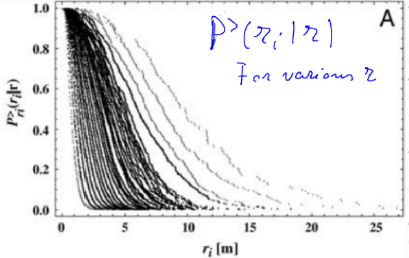
\includegraphics[width=0.8\textwidth]{\main/Images/tree_size.png}
    \caption{Plot of the \textit{accumulated} probabilities for $r_i$ for various tree sizes $r$.}
    \label{fig:tree_size}
\end{figure}

If the ansatz in (\ref{eqn:tree-ansatz}) is correct, then by rescaling the $x$ axis to $r_i/r^{2/3}$ we should see all curves \q{collapsing} into one. This indeed happens in fig. \ref{fig:tree-collapse}.

\begin{figure}[H]
    \centering
    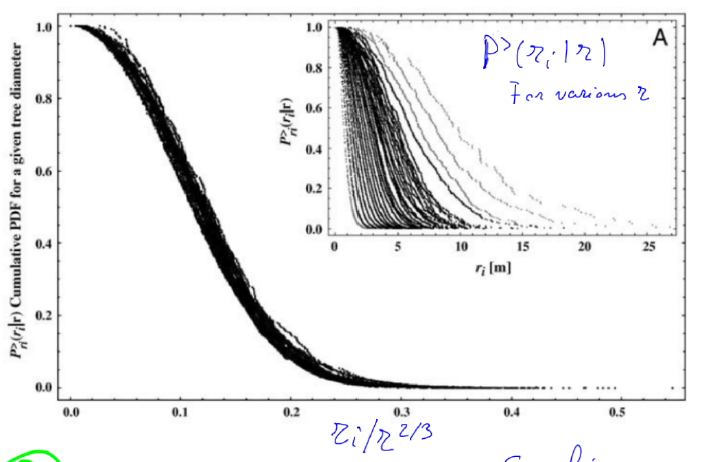
\includegraphics[width=0.8\textwidth]{\main/Images/tree-collapse.png}
    \caption{All curves from fig. \ref{fig:tree_size} collapse (approximately) into one when rescaling the $x$ axis according to ansatz (\ref{eqn:tree-ansatz})}
    \label{fig:tree-collapse}
\end{figure}

This means that there is some kind of \textit{emergent behaviour} in the forest: the distribution of tree sizes is not completely random, but exhibits a \textit{scaling behaviour}, which is similar to the one we studied in the Ising model. In a sense, the forest has \q{self-tuned} to a state \q{near criticality}. Yet, it is not clear \textit{why} this is the case - for example what is the evolutionary advantage in this kind of \q{self tuning}.

\begin{exo}[Plots]
    Plot the \textbf{specific heat} and the \textbf{susceptibility} as a function of $K$ at $h=0$ in the mean field approximation of the Ising Model with reduced Hamiltonian:
    \begin{align*}
        -\beta H = K \sum_{\langle x,y \rangle} \sigma_x \sigma_y + h \sum_x \sigma_x
    \end{align*}

    \medskip

    \textbf{Solution}. 
\end{exo}

\begin{exo}[Phase diagram]\label{exo:phase-diagram}
    Consider a variational free energy density of the form:
    \begin{align*}
        f_V(m,a,b,c) = a m^2 + b m^4 + cm^6 - hm
    \end{align*}
    where $m$ is the magnetization, $a$, $b$ and $c$ are coefficients, which are suitable functions of the temperature, and $h$ is proportional to the external magnetic field. $m$, $a$ and $b$ are allowed to be real numbers, whereas $c > 0$ to guarantee that $f_V$ is bounded from below. 
    \begin{enumerate}
        \item Determine \textit{analytically} the whole phase diagram in the $a$ - $b$ plane for a fixed value of $c$ and $h=0^+$, showing where the first and second order transitions occur.
        \item Sketch the form of the free energy density in the various phases and along the transition lines.
        \item Solve numerically the equation for the spontaneous magnetization.
    \end{enumerate}

    \medskip

    \textbf{Solution}. 
\end{exo}

\begin{exo}[Mean field IM]
    Consider an Ising Model in a $d$-dimensional hyper-cubic lattice with both nearest-neighbour ($\langle \cdot \rangle$) and $4$-spin ($[\cdot]$) interactions on the elementary squares of the lattice, with energy function given by:
    \begin{align*}
        - \beta H(\bm{\sigma}) = K \sum_{\mathclap{\langle x,y \rangle}} \sigma_x \sigma_y + L \sum_{\mathclap{[xyvz]}} \sigma_x \sigma_y \sigma_v \sigma_z
    \end{align*}
    where periodic boundary conditions are used, and $\sigma_x = \pm 1$ for every lattice node $x$.

    \medskip

    Use the mean field approximation to determine, in the thermodynamic limit:
    \begin{enumerate}
        \item The analytical expression, as a function of the magnetization $m$, of the variational free energy per node, $f_V(m,K,L)$, the entropy per node, $s(m,K,L)$, the mean energy per node $\epsilon(m,K,L)$ and the specific heat per node, $c(m,K,L)$.
        \item The phase diagram in the plane $K$ - $L$, with $K \geq 0$ and $L \geq 0$, specifying where the magnetization changes with continuity (second order phase transition), and where it changes with a discontinuity (first order phase transition).
    \end{enumerate}

    Notice that, while the whole second order transition line, including its end (the tri-critical point), can be determined analytically, the first order transition line has to be determined numerically.
\end{exo}

\begin{exo}[Scaling ansatz]
    Show that the scaling ansatz in equation (\ref{eqn:h-equation-state}, pag. \pageref{eqn:h-equation-state}) is equivalent to assume that $M(K,h)$ has the following homogeneous form in the vicinity of the critical point $(K_c, h_c) = (1/2d, 0)$:
    \begin{align*}
        |M(K,h)| = |t|^\beta g_{\pm} (h|t|^{-\beta \delta}) \qquad \beta = \frac{1}{2}, \> \delta=3 
    \end{align*}
    where $g_\pm$ is an odd function, i.e. $g_{\pm}(-x) = - g_{\pm}(x)$, and $g_+$ ($g_-$) is used when $t>0$ ($t<0$).
\end{exo}

\begin{exo}[Collapse plot]
    Minimize the variational free energy:
    \begin{align*}
        \beta \frac{F_V(m,K,h)}{N} = - Kd m^2 + \frac{1+m}{2} \ln \frac{1+m}{2} + \frac{1-m}{2} \ln \frac{1-m}{2} - hm    
    \end{align*}
    with respect to $m$ and determine where the minimum occurs ($M(K,h)$).

    Plot $M(K,h)$ as a function of $h$ for various values of $K > 1/(2d)$ and $K < 1/(2d)$, with several of them in the neighbourhood of $1/(2d)$. For the various curves so obtained, define $t \equiv (K_c - K)/K_c$, where $K_c \equiv 1/(2d)$, and verify the scaling ansatz (\ref{eqn:h-equation-state}) by plotting:
    \begin{align*}
        \frac{h}{M^3(K,h)} \text{ vs } \frac{|t|}{M^2(K,h)} \qquad (\delta = 3, \> \beta = \frac{1}{2} )
    \end{align*}
    What you should obtain is that the collapse shown in fig. \ref{fig:collapse_plot} is good only when both $|t|$ and $|h|$ are sufficiently small.

    Show that an alternative collapse can be obtained by plotting $|M(K,h)| |t|^{1/2}$ vs $|h| |t|^{-3/2}$. Notice that, according to exercise \ref{exo:phase-diagram}, one should obtain a collapsed curve for all $t \gtrsim 0$ (i.e. $K \lesssim K_c$) and a different one for all $t \lesssim 0$ (i.e. $K \gtrsim K_c$).

    The collapse quality deteriorates when $|h|$ and/or $|t|$ increase.

    \medskip

    \textbf{Solution}. 
\end{exo}

\begin{exo}[Scaling relations]
    Use the following scaling ansatz for the free energy density:
    \begin{align*}
        f(t,h) = |t|^{d \nu} \varphi(t|h|^{-1/\beta \delta})
    \end{align*}
    to deduce the scaling relations in (\ref{eqn:scaling-relations}, pag. \pageref{eqn:scaling-relations}):
    \begin{align*}
        \beta(\delta-1) = \gamma \qquad \beta(\delta+1) = 2 - \alpha \qquad d \nu -2 = \alpha
    \end{align*}
\end{exo}

%TODO Add exercise guide (non recorded lecture) end of 30/4 lecture

\chapter{Beyond Mean Field\\ and Universality}
Many years of study of phase transitions have shown that there are few \textit{types} of critical behaviours, meaning that \textbf{many systems} exhibit the \textbf{same kind} of \textbf{behaviour} near \textbf{criticality}.

\medskip

As an explicit example, a summary of the critical exponents for several \textit{classes} of models is shown in fig. \ref{fig:table-criticality}. 

\begin{figure}[H]
    \centering
    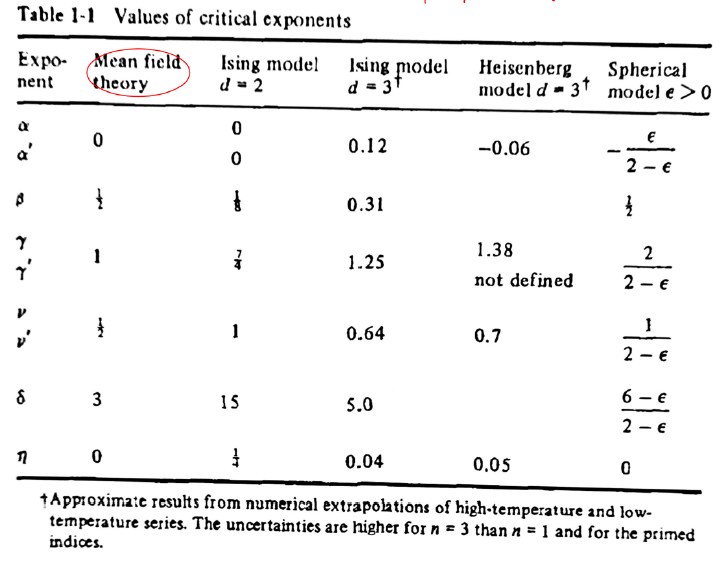
\includegraphics[width=0.8\textwidth]{\main/Images/table-criticality.png}
    \caption{Values of critical exponents for several models. As these exponents do not depend on all the details of each model, there is no need to fully specify each Hamiltonian. For example, the IM in $d=2$ could have more complex couplings between spins (other than the nearest neighbour ones we considered until now). Taken from \cite{renormalization}}
    \label{fig:table-criticality}
\end{figure}

Here there is no need to \textbf{fully specify} the \textbf{Hamiltonian} of each model: for instance, when talking about a Ising Model in $d=2$, the exponents are the same no matter how complex the spin couplings may be (for example, not only nearest neighbours may be interacting).

Moreover, if we consider higher and \textbf{higher dimensions} , the exponents \textbf{tend} to the values obtained in the \textbf{mean field} approximation. For example, $\delta$ is $15$ in $d=2$, and $5$ in $d=3$, which is closer to the MF value of $3$.

There is also a dependence on the \textbf{symmetries} of each model. As an example we may consider the Heisenberg model, a generalization of the IM in which each spin is a $3$-vector. Now the system is globally \textit{rotationally symmetric}, meaning that the symmetry group is $\mathrm{O}(3)$. In the Ising Model with \textit{binary} spins, the spin-flip symmetry is instead described by the $\mathbb{Z}_2$ group. So, even if the two models are studied in the same number of dimension (e.g. $d=3$), the scaling exponents will be different, as can be seen in fig. \ref{fig:table-criticality}. 

\medskip

From this analysis, we find that the critical exponents do not depend on the specificity of the Hamiltonian, but only on two \textit{general} characteristics:
\begin{itemize}
    \item The \textbf{dimensionality} of the model
    \item The \textbf{symmetries} of the Hamiltonian  
\end{itemize}

In the following, we will try to give some mathematical foundation to these arguments, mainly motivated by heuristics and intuition. A true formal proof, while possible (in some cases), would require a level of depth and sophistication well outside the scope of this course.

\medskip

In essence, the idea is to start by fixing a specific symmetry - for instance that of the Ising Model - and consider the \textit{most general} kind of Hamiltonian with that symmetry. The goal is to compute the partition function as a \textit{power series}, and demonstrate that, at least near criticality, the relevant coefficients are few, and depend only on the initial symmetry and the model's dimensionality.

\medskip

However, this kind of computation is impossible if we are dealing with \textit{discrete variables}, such as the \textit{binary} spins $\sigma_i = \pm 1$ of the IM, as in general there is no analytical way to compute the sum in the partition function. A way around this is to convert the model to \textit{continuous} variables, i.e. spins $\sigma_i \in \mathbb{R}$, making the partition function vanish for values $\varphi_x$ that are \q{far} from the discrete ones ($\pm 1$). This, along with some reasonable assumptions (such as translational invariance and short-range interactions) allows to expand $Z$ in series near criticality, and study its behaviour. 

\medskip

We can then search for the \textit{simplest} discrete model that is able to recreate the relevant coefficients in the $Z$ expansion, and thus provide a \q{minimal description} for the behaviour of entire \textit{classes} of systems.   

\section{From discrete to continuous variables}
Consider a Ising Model, with a general Hamiltonian including also more complex spin-spin interactions:
\begin{align}\label{eqn:H-complex}
    -\beta H(\bm{\sigma}) = \sum_{x,y} K_{xy} \sigma_x \sigma_y + \sum_{x,y,z,t} K_{xyzt} \sigma_x \sigma_y \sigma_z \sigma_t + \dots
\end{align}
The term $K_{xy}$ (and similarly the others) could include not only neighbouring spins, but also next-to-neighbouring spins and so on. One important constraint\marginpar{1. Symmetry} is to allow only interaction between an \textbf{even} number of spins, so that the Hamiltonian has still a \textit{spin-flip} symmetry:
\begin{align*}
    H(\bm{\sigma}) = H(-\bm{\sigma})
\end{align*}  
which is described by the cyclic group $\mathbb{Z}_2$.

\medskip

The partition function is given by:
\begin{align*}
    Z = \sum_{\{\bm{\sigma}\}} e^{-\beta H(\bm{\sigma})}
\end{align*}
This is a function of \textbf{discrete} binary variables $\sigma_x = \pm 1$. We can write it as a function of \textit{continuous} variables $\varphi_x$ by \textit{zeroing} all values where $\varphi_x \neq \pm 1$ with a Dirac delta:
\begin{align}\label{eqn:Z-delta}
    Z = \int_{\mathbb{R}^N} \Big[\prod_x \dd{\varphi_x} \delta(\varphi_x^2- 1)\Big] e^{-\beta H(\bm{\varphi})}
\end{align} 
The Dirac delta can then be written as the limit in which a smooth function (e.g. a gaussian) becomes more and more \q{peaked} (fig. \ref{fig:delta-peaks}):
\begin{align}\label{eqn:delta-limit}
    \delta(\varphi_x^2 - 1) = \lim_{\lambda \to +\infty} e^{- \lambda (\varphi_x^2 - 1)^2} \mathcal{N}(\lambda)
\end{align}
where $\mathcal{N}(\lambda)$ is a normalization constant. In fact, the integral of the $\delta$ is always fixed:
\begin{align}\label{eqn:delta-integral}
    \int_{-\infty}^{+\infty} \dd{\varphi} \delta(\varphi^2- 1) \underset{(a)}{=}  \int_{-\infty}^{+\infty} \dd{\varphi} \frac{\delta(\varphi-1) + \delta(\varphi+1)}{2|\varphi|} = \frac{1}{2|1|} + \frac{1}{2|-1|} = 1  
\end{align}
where in (a) we used the composition formula for the $\delta$:
\begin{align*}
    \delta(g(x)) = \sum_{i} \frac{\delta(x-x_i)}{|g'(x_i)|} 
\end{align*}
with the sum over all (simple) roots $x_i$ of $g(x)$.

\begin{figure}[H]
    \centering
    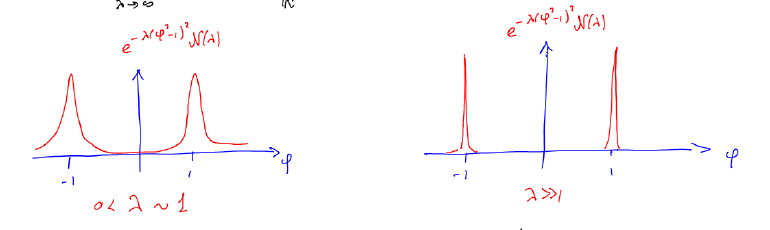
\includegraphics[width=0.9\textwidth]{\main/Images/delta-peaks.png}
    \caption{The $\delta(\varphi_x^2-1)$ can be seen as the limit of a smooth function with two peaks in $\pm 1$, which become more and more sharp as $\lambda \to +\infty$, while maintaining the area under the curve fixed to $1$.}
    \label{fig:delta-peaks}
\end{figure}

Imposing (\ref{eqn:delta-integral}) in (\ref{eqn:delta-limit}) leads to the following expression for the normalization $\mathcal{N}(\lambda)$:
\begin{align*}
    \mathcal{N}(\lambda) = \Big[\int_{-\infty}^{+\infty} \dd{\varphi} e^{-\lambda (\varphi^2-1)^2}\Big]^{-1}
\end{align*}

Then, substituting (\ref{eqn:delta-limit}) into the partition function (\ref{eqn:Z-delta}) we get:
\begin{align} \label{eqn:Z-limit}
    Z = \lim_{\lambda \to \infty} \mathcal{N}(\lambda)^N \int_{\mathbb{R}^N} \Big[\prod_x \dd{\varphi_x} \Big] \exp\left(-\beta H (\bm{\varphi}) - \lambda\sum_x (\varphi_x^2-1)^2 \right)
\end{align}

Experimentally, we observe that near criticality the details of the system do not matter for describing its behaviour - and so we expect that the system with finite $\lambda$ (e.g. $\lambda \sim 1$) will behave \textit{similarly} to the one with $\lambda \to +\infty$. Mathematically, studying the first case allows us to deal with \textit{smooth} functions.

\medskip

So, removing the limit from (\ref{eqn:Z-limit}) is equivalent to study the following Hamiltonian:
\begin{align*}
    -\beta H_{\mathrm{tot}}(\bm{\varphi}) = -\beta H(\bm{\varphi}) - \lambda\sum_x (\varphi_x^2 -1)^2 
\end{align*}

Let's\marginpar{2. Translational invariance} now assume that all spin-spin interactions are \textbf{translationally invariant}, meaning that the interaction terms $K_{xy}$, $K_{xyzt}$ and so on are all functions of \textit{distances}.

\medskip

Explicitly, let's focus for instance on $K_{xy}$. Translational invariance means that we can write it as:
\begin{align*}
    K_{xy} = K_2(\bm{r}_x - \bm{r}_y)
\end{align*}
for some function $K_2$. Then, due to the $\mathbb{Z}_2$ symmetry, $K_2(\bm{r}_x - \bm{r}_y) = K_2(\bm{r}_y - \bm{r}_x)$. In fact, if the two spins are the same (both $+1$ or $-1$), then exchanging them will not make any difference. If they are different, i.e. one $+1$ and the other $-1$, exchanging them is equivalent to a \textit{spin-flip}, and so the result will still be the same. 

Thus, if we rewrite $\bm{r} = \bm{r}_x - \bm{r}_y = \bm{n} a$, with $\bm{n} \in \mathbb{Z}^d$, then $K_2(\bm{r})$ is an \textbf{even} function, and depends only on $\norm{\bm{r}}$ due to translational invariance.

This means that all averages of only one component of $\bm{r}$ are zero:
\begin{align}\label{eqn:r-average}
    \sum_{\bm{r}} K_2(\norm{\bm{r}}) r_\alpha = 0 \qquad \alpha=1,\dots,d
\end{align}
because $K_2$ is even, while $r_\alpha$ is odd.

\medskip

We also assume interactions to be \textbf{short range}\marginpar{3. Short range interactions}. This means that the average of two components of $\bm{r}$ is proportional to $a^2$: 
\begin{align}\label{eqn:rr-average}
    \sum_{\bm{r}} K_2(\norm{\bm{r}}) r_\alpha r_\beta = \frac{\delta_{\alpha \beta}}{d}  \sum_{\bm{r}} K_2(\norm{\bm{r}}) \norm{\bm{r}}^2 \propto a^2 < \infty
\end{align} 
The $\delta_{\alpha \beta}$ comes from the fact that we expect different directions to be independent (\textbf{isotropy}), and the $d$ is just a normalization for the Kronecker delta.

\medskip

Similar relations are expected to hold for all higher order interaction terms ($K_{xyzt}$ and so on).

\medskip

With all these assumptions, we can simplify the Hamiltonian (\ref{eqn:H-complex}). For instance, the $K_{xy}$ term becomes:
\begin{align*}
    \sum_{xy} K_2(\bm{r}_x - \bm{r}_y) \varphi(\bm{r}_x) \varphi(\bm{r}_y)
\end{align*}
with $\varphi(\bm{r}_x) \equiv \varphi_x$ and $\varphi(\bm{r}_y) \equiv \varphi_y$. In this notation, $x$ and $y$ are \textit{numeric} indices for the spins, and $\bm{r}_x$, $\bm{r}_y \in \mathbb{Z}^d a$ are their positions in the lattice. Then $\varphi(\bm{r}_x) \in \mathbb{R}$ refers to the \textit{spin} of the cell $x$ at position $\bm{r}_x$. 

\medskip

Changing variables to $\bm{r} = \bm{r}_x - \bm{r}_y$ leads to:
\begin{align*}
    \sum_y \varphi(\bm{r}_y) \sum_{\bm{r}} K_2(\bm{r}) \varphi(\bm{r}_y + \bm{r})
\end{align*}
Now we use the fact that $K_2$ is \textbf{short range}, and so the dominant contributions to the sum are the ones with small $\bm{r}$. Near \textbf{criticality},\marginpar{4. Criticality} we expect the correlation length to diverge, meaning that spins that are far apart can be highly correlated. Qualitatively, this leads to spin configurations that are \q{smooth}, in the sense that neighbouring spins are similarly aligned. Mathematically, this allows us to treat $\varphi(\bm{r})$ as a smooth function of the position $\bm{r}$, and in particular to expand it in series around $\bm{r}=\bm{0}$:\marginpar{\vspace{29em}5. Continuum limit}
\begin{align*}
    \sum_y \varphi(\bm{r}_y) \sum_{\bm{r}} K_2(\bm{r}) \left[\varphi(\bm{r}_y) + \sum_{\alpha=1}^d r_\alpha \pdv{r_\alpha} \varphi(\bm{r})\Big|_{\bm{r} = \bm{r}_y} + \frac{1}{2} \sum_{\alpha, \beta=1}^d r_\alpha r_\beta \pdv[2]{}{r_\alpha}{r_\beta} \varphi(\bm{r})\Big|_{\bm{r} = \bm{r}_y} + \dots \right] =\span\\
    \shortintertext{We can then exchange some of the sums to use (\ref{eqn:r-average}) and (\ref{eqn:rr-average}):}
    &= \sum_y \varphi(\bm{r}_y) \underbrace{\sum_{\bm{r}} K_2(\bm{r})}_{c_2}  \varphi(\bm{r}_y) + \sum_y \varphi(\bm{r}_y) \sum_{\alpha=1}^d \underbrace{\Big(\sum_{\bm{r}} K_2(\bm{r}) r_\alpha \Big)}_{0 \> (\ref{eqn:r-average})} {\pdv{\varphi}{r_\alpha}}(\bm{r}_y) + \\
    &\quad \> +\sum_y \varphi(\bm{r}_y)\sum_{\alpha,\beta=1}^d \underbrace{\Big(\sum_{\bm{r}} \frac{r_\alpha r_\beta }{2} K_2(\bm{r}) \Big)}_{\propto \delta_{\alpha \beta} a^2 \> (\ref{eqn:rr-average})} {\pdv[2]{\varphi}{r_\alpha}{r_\beta}} (\bm{r}_y) + \dots =\\
    \shortintertext{And inserting a coefficient $c_3$ to account for the proportionality:}
    &= c_2 \sum_y \varphi(\bm{r}_y)^2 + c_3 a^2 \sum_{y} \varphi(\bm{r}_y) \underbrace{\sum_{\alpha=1}^d {\pdv[2]{\varphi}{r_\alpha}} (\bm{r}_y)}_{\nabla^2 \varphi(\bm{r}_y)}  =\\
    &= c_2 \sum_y \varphi(\bm{r}_y)^2 + c_3 a^2 \sum_y \varphi(\bm{r}_y) \nabla^2(\bm{r}_y)
    \intertext{Taking the \textbf{continuum limit} $a \to 0$ (an \q{infinitely dense} lattice) the summation becomes an integral. We then \textit{rescale} the integration variable from $\bm{r}_y = \bm{y} a$, resulting in an additional $a^{-d}$ factor, so that the integrand is adimensional:}
    &\underset{\mathclap{a \to 0}}{=} \> \int_{\mathbb{R}^d} \dd[d]{\bm{y}} a^{-d} \left[c_2 \varphi(a \bm{y})^2 + \hlc{Yellow}{c_3 a^2 \varphi(a \bm{y}) \nabla^2 \varphi(a \bm{y}) }+ \dots \right] =
    \intertext{Finally, integrating by parts two times the highlighted term, and ignoring the resulting surface terms, leads to:}
    &= \int_{\mathbb{R}^d} \dd[d]{\bm{y}} a^{-d} \left[c_2 \varphi^2 (a\bm{y}) - c_3 a^2 (\nabla \varphi(a\bm{y}))^2 + \dots \right]
\end{align*} 

A similar procedure can be done also for the other interaction terms. For instance, consider the \textit{quartic} term:
\begin{align*}
    \sum_{x,y,z,t} K_{xyzt} \varphi(\bm{r}_x) \varphi(\bm{r}_y) \varphi(\bm{r}_z) \varphi(\bm{r}_t)
\end{align*} 
Translational invariance implies that:
\begin{align*}
    K_{xyzt} = K_4(\bm{r}_x-\bm{r}_y, \bm{r}_z-\bm{r}_y, \bm{r}_t-\bm{r}_y)
\end{align*}
And so we can rewrite the term in the Hamiltonian as follows:
\begin{align*}
    \sum_{xyzt} K_{xyzt} \varphi(\bm{r}_x) \varphi(\bm{r}_y) \varphi(\bm{r}_z) \varphi(\bm{r}_t) =\\
    \underset{\mathclap{\substack{
        \bm{r}_1 \equiv \bm{r}_x - \bm{r}_y\\
        \bm{r}_2 \equiv \bm{r}_z - \bm{r}_y\\
        \bm{r}_3 \equiv \bm{r}_t - \bm{r}_y
    }}}{=}\quad\>  \sum_y \varphi(\bm{r}_y) \sum_{\bm{r}_1, \bm{r}_2, \bm{r}_3} K_4(\bm{r}_1, \bm{r}_2, \bm{r}_3) \varphi(\bm{r}_y + \bm{r}_1) \varphi(\bm{r}_y + \bm{r}_2) \varphi(\bm{r}_y + \bm{r}_3)\span
\end{align*}
And then expand around $\bm{r}_1, \bm{r}_2, \bm{r}_3 = \bm{0}$.

\medskip

After all these manipulations, the Hamiltonian will look like:
\begin{align*}
    - \beta H_{\mathrm{tot}}(\bm{\varphi}) = \int_{\mathbb{R}^d} \dd[d]{\bm{y}} a^{-d} \Big[&-\hlc{Yellow}{c_3 a^2 (\nabla \varphi)^2 }+ \hlc{ForestGreen}{\hat{c}_2 \varphi^2 }+ \hlc{SkyBlue}{\hat{c}_4 \varphi^4 }+ \dots \\
    &+\hlc{SkyBlue}{d_2 a^2 (\nabla \varphi)^2 }+ \dots \Big]
\end{align*}
The yellow term comes from the binary interactions, the blue ones from the quartic interactions, and the green includes contributions from both of them.

\medskip

As $\varphi \in \mathbb{R}$, through a change of variables we can \textit{fix} one of the coefficients - for example\footnote{The choice of which coefficient to fix is arbitrary. At the end, we will be interested in the \q{relative order of magnitude} of the coefficients} $c_3$ to $1/2$. So we consider the transformation $\varphi = \zeta \phi$, with $\zeta \in \mathbb{R}$ constant such that:
\begin{align*}
    c_3 a^{2-d} (\nabla \varphi)^2 = c_3 a^{2-d}\zeta^2(\nabla \phi)^2 \overset{!}{=}  \frac{1}{2} (\nabla \phi)^2 \Rightarrow \zeta^2 = \frac{a^{d-2}}{c_3} 
\end{align*}  

After this, the Hamiltonian becomes:
\begin{align}\label{eqn:continuum-limit}
    -\beta H_{\mathrm{tot}}(\bm{\varphi}) \equiv -\beta \mathcal{H}(\bm{\phi}) = - \int_{\mathbb{R}^d} \dd[d]{\bm{y}} \Big[&\frac{1}{2}(\nabla \phi)^2 + \frac{\mu}{2} \phi^2 + g_4 \phi^4 + g_6 \phi^6 + \dots +\\
    &+ f_2 (\nabla \phi)^2 \phi^2 + \dots \Big]
\end{align}
It is not important to specify exactly the dependence of these new coefficients $\mu, g_4, g_6, f_2, \dots$ on the old ones $c_3, \hat{c}_2, \hat{c}_4, d_2, \dots$. For now, let's just observe their order on $a$:
\begin{align*}
    \mu \propto a^{-2}; \> g_4 \propto a^{d-4}; \> g_6 \propto a^{2(d-3)}; \> g_8 \propto a^{3d-8}; \> f_2 \propto a^{d-2}
\end{align*}
%TODO How to find them? 22:25

When taking the continuum limit $a \to 0$, $\mu$ always diverges, while the other coefficients either vanish or diverge\footnote{In fact, we take the continuum limit in the first place just to quantify the relative importance of these coefficients} depending on $d$. For instance:
\begin{itemize}
    \item $d > 4$: only $\mu$ is diverging
    \item $3 < d < 4$: $\mu$ and $g_4$ diverge
    \item $8/3 < d < 3$: $\mu, g_4, g_6$ diverge
\end{itemize}
In particular, this means that for $d > 4$, a purely gaussian model can be used to describe the system, and it's able to capture all the behaviour of the system near criticality:
\begin{align*}
    -\beta H_G(\bm{\phi}) = - \int_{\mathbb{R}^d}\dd[d]{\bm{x}} h_g(\bm{\phi}, \partial_\alpha \bm{\phi}) \qquad h_G(\bm{\phi}) = \frac{1}{2}\left[(\nabla \phi)^2 + \bm{\phi}^2 \right] 
\end{align*}

This is the essence of \textbf{universality}: a critical system can be described with few parameters, which depend only on the symmetry and the dimensionality (assuming short-range interactions).   

\medskip

From a physical point of view, we are interested only in the $d=3$ (general systems) and $d=2$ cases (interfaces/surfaces of systems). However, all other possibilities are still relevant theoretically. In particular, the concept of \textit{fractional dimensions} enables \textit{perturbative expansions}. The idea is that for $d \lesssim 4$ we can write $d = 4 - \epsilon$, with $\epsilon \approx 0$. This means that $g_4$ is \q{less important} than $\mu$, and can be treated perturbatively starting from a Gaussian model, leading to results that agree well with experiments. In particular, this has lead to very powerful \textit{renormalization group techniques}, which are able to shed light onto the so-called \q{universality classes}, i.e. very general \q{types} of models with similar critical behaviour.

\section{Back to the discrete world}
In summary, the continuum limit $a \to 0$ has shown to us that only a \textbf{finite number of terms} in the \textbf{Hamiltonian} are \textbf{important}. 

Thus, a \textbf{discrete model} with just the \q{right complexity} so that its continuum limit matches just the first terms of (\ref{eqn:continuum-limit}) is enough to describe \textit{all the systems} in the same \textit{universality class} near criticality!

\medskip

One such example is the Nearest Neighbour Ising Model that we have already studied. In the same universality class we find the \q{Next Neighbour} Ising Model, in which a spin may interact with a \textit{neighbour} of its \textit{neighbours} (fig. \ref{fig:n-nIM}). Explicitly, the Hamiltonian is given by:
\begin{align*}
    -\beta H(\bm{\sigma}) = \textcolor{Blue}{K \sum_{\langle x,y \rangle} \sigma_x \sigma_y} + \textcolor{ForestGreen}{L \sum_{\langle \langle x,y \rangle \rangle} \sigma_x \sigma_y}
\end{align*}
where the second sum is over all $x$ and $y$ that \textit{share} a neighbour $z$ (i.e. that are \q{neighbours of neighbours}).

\begin{figure}[H]
    \centering
    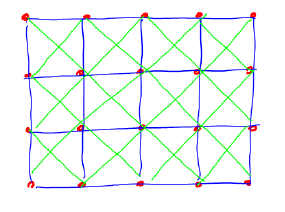
\includegraphics[width=0.5\textwidth]{\main/Images/n-nIM.png}
    \caption{Diagram of the interactions in a Next Neighbour Ising Model. Spins in the lattice are represented as red dots, the usual \textit{nearest neighbour} interactions are in \textcolor{Blue}{blue}, and the \textit{next neighbour} interactions are in \textcolor{ForestGreen}{green}.}
    \label{fig:n-nIM}
\end{figure}

Results from renormalization group theory show that the phase diagram of this kind of model is that of fig. \ref{fig:critical-n-nIM}.

\begin{figure}[H]
    \centering
    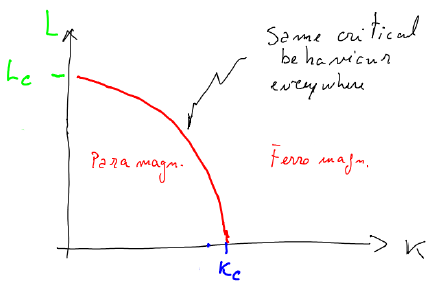
\includegraphics[width=0.8\textwidth]{\main/Images/critical-n-nIM.png}
    \caption{Phase diagram of the Next Neighbour Ising Model.}
    \label{fig:critical-n-nIM}
\end{figure}

When the system is near criticality (i.e. along the red line of fig. \ref{fig:critical-n-nIM}) its behaviour is described by the \textbf{same set of critical exponents} that appear in the Nearest Neighbour Ising Model we previously examined. 

\medskip

Let's add \textit{another term} to the Hamiltonian, describing \textit{quartic} interactions:
\begin{align}\label{eqn:H-complicated}
    -\beta H(\bm{\sigma}) = \textcolor{Blue}{K \sum_{\langle x,y \rangle} \sigma_x \sigma_y} + \textcolor{ForestGreen}{L \sum_{\langle \langle x,y \rangle \rangle} \sigma_x \sigma_y} + \textcolor{Cyan}{M \sum_{[xyzt]} \sigma_x \sigma_y \sigma_z \sigma_t}
\end{align}
 
\begin{figure}[H]
    \centering
    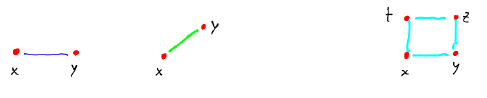
\includegraphics[width=0.5\textwidth]{\main/Images/interactions.png}
    \caption{Types of interactions in (\ref{eqn:H-complicated})}
    \label{fig:interactions}
\end{figure}

In this case, the phase diagram is shown in fig. \ref{fig:complicated-phases}. Near the \textit{red surface}, at which a second order transition happens, the system's behaviour is again described by the same critical exponents that appear in the Nearest Neighbour Ising Model! They are only different when crossing the \textit{green surface} (corresponding to a first order transition, for which there is no universality in principle) and the boundary between the two surfaces, called the \textit{tri-critical line} (which belongs to a \textit{different} universality class).   


\begin{figure}[H]
    \centering
    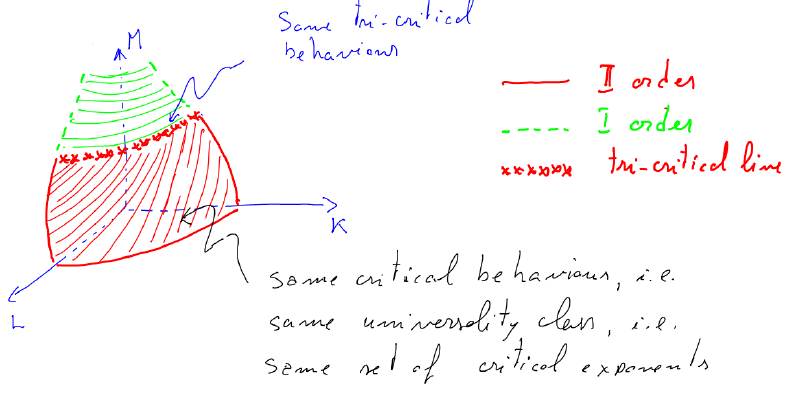
\includegraphics[width=0.8\textwidth]{\main/Images/complicated-phases.png}
    \caption{Phase diagram for the model (\ref{eqn:H-complicated})}
    \label{fig:complicated-phases}
\end{figure}

 



\end{document}
